\documentclass{article}

\usepackage{graphicx}
\usepackage{tikz}
\usepackage{tikzsymbols}
\usetikzlibrary{calc,patterns,shapes.geometric}
\pagestyle{empty}
\usepackage[margin=0pt]{geometry}
\geometry{papersize={14in,12in}}

\def\centerarc[#1](#2)(#3:#4:#5){\draw[#1] ($(#2)+({#5*cos(#3)},{#5*sin(#3)})$) arc (#3:#4:#5);}

\begin{document}
	\begin{figure}
		\centering
		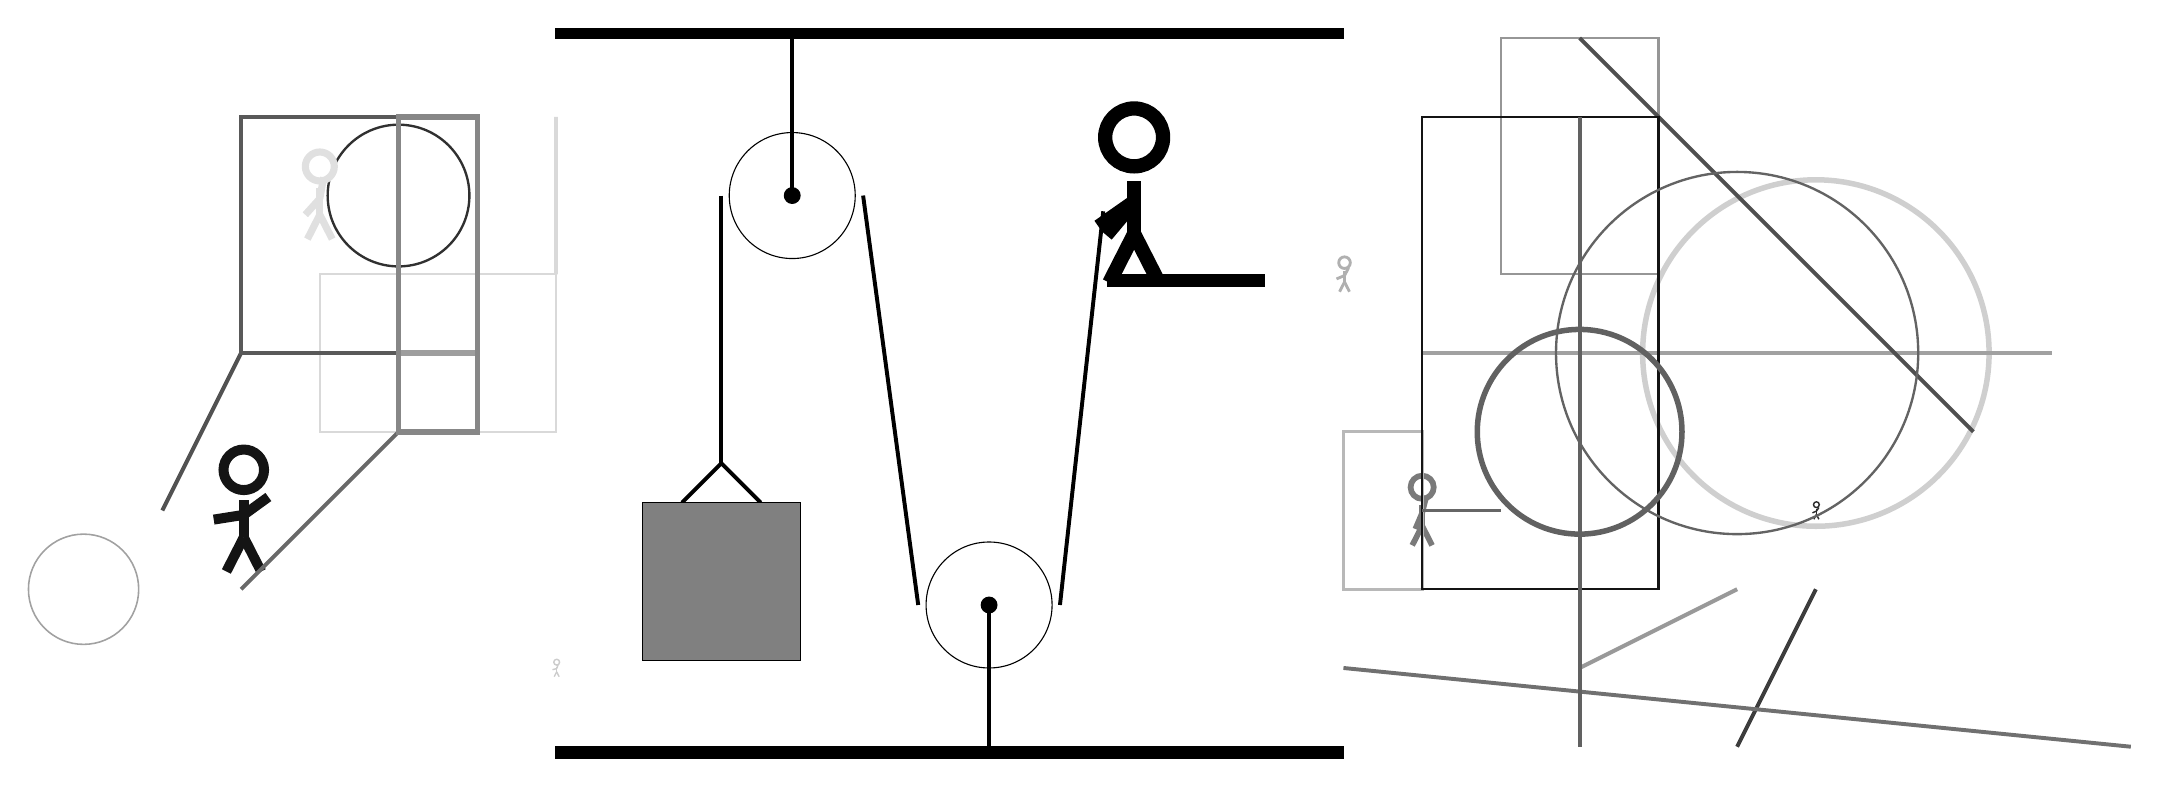
\begin{tikzpicture}
			%%%%% START %%%%%
			
			\draw[fill=black] (-2, 9) rectangle (8, 9.125);
			
			\draw (3.5, 1.8) circle (0.8);
			\draw[fill=black] (3.5, 1.8) circle (0.1);
			\draw[line width=0.5mm] (3.5, 1.8) -- (3.5, 0);
			
			\draw (1, 7) circle (0.8);
			\draw[fill=black] (1, 7) circle (0.1);
			\draw[line width=0.5mm] (1, 9) -- (1, 7);
			
			\draw[line width=0.5mm](-0.4, 3.1) --  (0.1, 3.6) -- (0.6, 3.1);
			\draw[fill=black!50] (-0.9, 3.1) rectangle (1.1, 1.1);
			
			\draw[line width=0.5mm](0.1, 7) -- (0.1, 3.6);
			\centerarc[line width=0.5mm](1, 7)(180:0:0.9)
			\draw[line width=0.5mm](1.9, 7) -- (2.6, 1.8);
			\centerarc[line width=0.5mm](3.5, 1.8)(180:360:0.9)
			\draw[line width=0.5mm](4.4, 1.8) -- (4.95, 6.8);
			
			\draw[line width=0.7mm, color=black!38] (-4, 5) rectangle (-3, 4);
			
			\node[line width=0.4mm, color=black!31] at (8, 6) {\Strichmaxerl[2][23][62]};
			\draw[line width=0.2mm, color=black!15] (-2, 6) rectangle (-5, 4);
			\node[line width=0.5mm, color=black!92] at (-6, 3) {\Strichmaxerl[7][9][36]};
			
			\draw [line width=0.7mm, color=black!19](14, 5) circle (2.2);
			\node[line width=0.5mm, color=black!52] at (9, 3) {\Strichmaxerl[4][67][76]};
			\node[line width=0.5mm, color=black!83] at (14, 3) {\Strichmaxerl[1][23][55]};
			\draw[line width=0.5mm, color=black!37](9, 5) -- (17, 5);
			\draw[line width=0.5mm, color=black!40](11, 1) -- (13, 2);
			\draw [line width=0.3mm, color=black!81](-4, 7) circle (0.9);
			
			\draw[line width=0.4mm, color=black!28] (8, 4) rectangle (9, 2);
			\draw[line width=0.5mm, color=black!76](13, 0) -- (14, 2);
			\draw[line width=0.5mm, color=black!68](-7, 3) -- (-6, 5);
			
			\draw[line width=0.5mm, color=black!56](8, 1) -- (18, 0);
			\draw[line width=0.3mm, color=black!54] (9, 5) rectangle (9, 5);
			\draw[line width=0.3mm, color=black!23] (-3, 7) rectangle (-3, 6);
			
			\draw[line width=0.3mm, color=black!41] (10, 6) rectangle (12, 9);
			
			\node[line width=0.6mm, color=black!12] at (-5, 7) {\Strichmaxerl[5][48][80]};
			\draw[line width=0.5mm, color=black!69](11, 9) -- (16, 4);
			\draw[line width=0.3mm, color=black!92] (9, 8) rectangle (12, 2);
			\draw[line width=0.5mm, color=black!65] (-4, 8) rectangle (-6, 5);
			
			\draw[line width=0.5mm, color=black!59](-4, 4) -- (-6, 2);
			\node[line width=0.4mm, color=black!20] at (-2, 1) {\Strichmaxerl[1][14][70]};
			\draw[line width=0.7mm, color=black!47] (-3, 8) rectangle (-4, 4);
			\draw[line width=0.5mm, color=black!62](11, 8) -- (11, 0);
			
			\draw [line width=0.7mm, color=black!62](11, 4) circle (1.3);
			
			\draw[line width=0.4mm, color=black!15] (-2, 6) rectangle (-2, 8);
			\draw[line width=0.4mm, color=black!60] (9, 3) rectangle (10, 3);
			\draw [line width=0.3mm, color=black!61](13, 5) circle (2.3);
			
			\draw [line width=0.2mm, color=black!37](-8, 2) circle (0.7);
			
			\node at (5.3, 7) {\Strichmaxerl[10][35][-130]};
			\draw[fill=black] (5, 6) rectangle (7, 5.85);
			
			\draw[fill=black] (-2, 0) rectangle (8, -0.15);
			
			%%%%% END %%%%%
		\end{tikzpicture}
	\end{figure}	
\end{document}